\documentclass[oneside,listof=totoc]{scrbook}

% PENGATURAN
% Pengaturan ukuran kertas dan margin
\usepackage{geometry}
\geometry{
  a4paper,
  lmargin=40mm,
  rmargin=30mm,
  tmargin=40mm,
  bmargin=30mm
}

% Pengaturan jarak antar baris
\usepackage{setspace}
\linespread{1.5}
\newcommand\tab[1][1cm]{\hspace*{#1}}

% Pengaturan font
\usepackage{fontspec}
\setmainfont{Times New Roman}

% Pengaturan daftar isi, daftar gambar, daftar tabel, daftar pustaka
\usepackage{hyperref}
\hypersetup{
    colorlinks=true,
    linkcolor=black,
    filecolor=black,
    urlcolor=blue,
}
\usepackage{hanging}
\setuptoc{toc}{totoc}
\usepackage[titles]{tocloft}
\setlength{\cftchapnumwidth}{42pt}
\setlength{\cftsecnumwidth}{27pt}
\setlength{\cfttabnumwidth}{49pt}
\setlength{\cftfignumwidth}{62pt}
\renewcommand{\cftchappresnum}{\chaptername\ }
\renewcommand{\cftchapdotsep}{\cftdotsep}
\renewcommand{\cftchapfont}{\normalfont\bfseries}
\renewcommand{\cfttabpresnum}{\tablename\ }
\renewcommand{\cfttabfont}{\normalfont\bfseries}
\renewcommand{\cftfigpresnum}{\figurename\ }
\renewcommand{\cftfigfont}{\normalfont\bfseries}
\renewcommand{\contentsname}{DAFTAR ISI}
\renewcommand{\listfigurename}{DAFTAR GAMBAR}
\renewcommand{\listtablename}{DAFTAR TABEL}

% Pengaturan gambar, label, caption, dan items
\usepackage{enumitem}
\usepackage{pgf,tikz}
\usepackage{caption}
\captionsetup[figure]{labelsep=space}
\renewcommand{\thefigure}{\arabic{chapter}.\arabic{figure}}
\renewcommand{\figurename}{\bfseries{Gambar}}
\renewcommand{\tablename}{\bfseries{Tabel}}
\renewcommand{\labelitemi}{\bfseries{--}}

% Pengaturan tabel
\captionsetup[table]{labelsep=space}
\renewcommand{\thetable}{\arabic{chapter}.\arabic{table}}
\usepackage{color, colortbl}
\definecolor{Gray}{gray}{0.7}
\usepackage{array}
\newcolumntype{L}[1]{>{\raggedright\let\newline\\\arraybackslash\hspace{0pt}}m{#1}}
\newcolumntype{C}[1]{>{\centering\let\newline\\\arraybackslash\hspace{0pt}}m{#1}}
\newcolumntype{R}[1]{>{\raggedleft\let\newline\\\arraybackslash\hspace{0pt}}m{#1}}

% Pengaturan bab dan subbab
\renewcommand{\chaptername}{BAB}
\renewcommand{\thechapter}{\Roman{chapter}}
\renewcommand{\thesection}{\arabic{chapter}.\arabic{section}}
\renewcommand{\thesubsection}{\arabic{chapter}.\arabic{section}.\arabic{subsection}}
\usepackage{titlesec}
\titleformat{\chapter}[display]
  {\normalsize\bfseries\centering}{\chaptertitlename\ \thechapter}{0pt}{}
  \titlespacing*{\chapter}{0pt}{-\topskip}{0pt}
\titleformat{\section}
  {\normalsize\bfseries}{\thesection}{12pt}{}
\usepackage{indentfirst}
\setlength{\parindent}{25pt}

% Pengaturan nomor halaman (konfigurasi pada masing-masing matter)
\usepackage{fancyhdr}

% Global variabel (tahun, nama, nim, dll)
\newcommand{\JudulLaporanKP}{JUDUL LAPORAN DALAM BAHASA INDONESIA \\ DITULIS SECARA SIMETRIS}
\newcommand{\NamaMahasiswa}{Nama Mahasiswa}
\newcommand{\NIM}{12.34.567}
\newcommand{\NamaDosenPembimbing}{Nama Dosen Pembimbing}
\newcommand{\NIDNDosenPembimbing}{NIDN 1234567890}
\newcommand{\NamaDosenPenguji}{Nama Dosen Penguji}
\newcommand{\NIDNDosenPenguji}{NIDN 1234567890}
\newcommand{\HariPembuatan}{Hari}
\newcommand{\TanggalPembuatan}{00}
\newcommand{\BulanPembuatan}{Bulan}
\newcommand{\TahunPembuatan}{2020}

\begin{document}

% FRONT MATTER
\frontmatter
\pagestyle{plain}

% Halaman: JUDUL
\clearpage
\thispagestyle{empty}

\begin{center}
  \normalsize{\textbf{LAPORAN KERJA PRAKTIK}\\
  \vspace{1.0cm}
  \textbf{\JudulLaporanKP}}
\end{center}

\vspace{3.0cm}

\begin{minipage}{12.2cm}
  \centering
    
\includegraphics[width=4.20cm]{gambar/logo_um}
\end{minipage}

\vspace{2.5cm}

\begin{center}
  \normalsize{Disusun oleh:}\\
  \vspace{0.2cm}
  \begin{minipage}{\textwidth}
    \begin{center}
      \begin{tabular}{l r l}
        \textbf{Nama} & : & \textbf{\NamaMahasiswa}\\
        \textbf{NIM}  & : & \textbf{\NIM}
      \end{tabular}
    \end{center}
  \end{minipage}
\end{center}

\vspace{3.0cm}

\begin{center}
  \normalsize{\textbf{PROGRAM STUDI INFORMATIKA-S1}}\\
  \normalsize{\textbf{FAKULTAS ILMU KOMPUTER}}\\
  \normalsize{\textbf{UNIVERSITA MULIA}}\\
  \normalsize{\textbf{BALIKPAPAN}}\\
  \normalsize{\textbf{\TahunPembuatan}}
\end{center}

% Halaman: SUB JUDUL
\chapter{LAPORAN KERJA PRAKTIK}

\vspace{1.0cm}

\begin{center}
  \normalsize{\textbf{\JudulLaporanKP}}
\end{center}

\vspace{0.5cm}

\begin{center}
  \normalsize{Diajukan untuk Memenuhi Salah Satu Syarat}\\
  \normalsize{Mata Kuliah Kerja Praktik Jenjang - S1}\\
  \normalsize{Program Studi Informatika}\\
\end{center}

\vspace{1.5cm}

\begin{minipage}{12.2cm}
  \centering
    
\includegraphics[width=4.20cm]{gambar/logo_um}
\end{minipage}

\vspace{1.5cm}

\begin{center}
  \normalsize{Disusun oleh:}\\
  \vspace{0.2cm}
  \begin{minipage}{\textwidth}
    \begin{center}
      \begin{tabular}{l r l}
        \textbf{Nama} & : & \textbf{\NamaMahasiswa}\\
        \textbf{NIM}  & : & \textbf{\NIM}
      \end{tabular}
    \end{center}
  \end{minipage}
\end{center}

\vspace{2.0cm}

\begin{center}
  \normalsize{\textbf{PROGRAM STUDI INFORMATIKA-S1}}\\
  \normalsize{\textbf{FAKULTAS ILMU KOMPUTER}}\\
  \normalsize{\textbf{UNIVERSITA MULIA}}\\
  \normalsize{\textbf{BALIKPAPAN}}\\
  \normalsize{\textbf{\TahunPembuatan}}
\end{center}

% Halaman: LEMBAR PENGESAHAN
\chapter{LEMBAR PENGESAHAN}

\vspace{0.5cm}

\begin{center}
  \normalsize{\textbf{\JudulLaporanKP}}
\end{center}

\vspace{0.1cm}

\begin{center}
  \linespread{1.0}
  \normalsize{Diajukan untuk Memenuhi Salah Satu Syarat\\
  Mata Kuliah Kerja Praktik Jenjang - S1\\
  Program Studi Informatika}
\end{center}

\vspace{1.5cm}

\begin{center}
  \textbf{\NamaMahasiswa}\\
  \textbf{\NIM}
\end{center}

\vspace{0.5cm}

\begin{center}
  \linespread{1.0}
  \normalsize{Telah Diperiksa dan Diujikan Sebagai Laporan Kerja Praktik\\
  Program Studi Informatika\\
  Universitas Mulia Balikpapan\\
  pada \HariPembuatan, \TanggalPembuatan\ \BulanPembuatan\ \TahunPembuatan}
\end{center}

\vspace{1.5cm}

\begin{minipage}{\textwidth}
  \tab[0.5cm]\textbf{Pembimbing} \tab[5.6cm] \textbf{Penguji}\\
  \vspace{1.3cm}\\
  \linespread{1.0}
  \normalsize{\tab[0.5cm]\textbf{\underline{\NamaDosenPembimbing}} \tab[3.4cm] \textbf{\underline{\NamaDosenPenguji}}\\
  \tab[0.5cm]\textbf{\NIDNDosenPembimbing} \tab[4.65cm] \textbf{\NIDNDosenPenguji}}
\end{minipage}

\vspace{1.5cm}

\begin{center}
  \linespread{1.0}
  \normalsize{Balikpapan, \TanggalPembuatan\ \BulanPembuatan\ \TahunPembuatan\\
  \textbf{Ketua Program Studi Informatika-S1}}
\end{center}
\vspace{1.3cm}
\begin{center}
  \linespread{1.0}
  \normalsize{\textbf{\underline{J a m a l, S.Kom., M.Kom.}}\\
  \textbf{NIDN 11020574}}
\end{center}

% Halaman: KATA PENGANTAR
\chapter{KATA PENGANTAR}
\vspace{0.5cm}

Bagian ini berisi pernyataan resmi yang ingin disampaikan oleh penulis kepada pihak lain, misalnya ucapan terima kasih kepada Dosen Pembimbing, Dosen Penguji, dan semua pihak yang terkait dalam penyelesaian Kerja Praktik (KP) termasuk orang tua dan penyandang dana.

Nama harus ditulis secara lengkap termasuk gelar akademik dan harus dihindari ucapan terima kasih kepada pihak yang tidak terkait. Bahasa yang digunakan harus mengikuti kaidah Bahasa Indonesia yang baku.

Bagian ini tidak perlu dituliskan hal-hal yang bersifat ilmiah. Kata Pengantar diakhiri dengan mencantumkan kota dan tanggal penulisan diikuti di bawahnya dengan kata “Penulis” tanpa perlu menyebutkan nama dan tanda tangan.

\vspace{1.0cm}

\noindent{Balikpapan, \TanggalPembuatan\ \BulanPembuatan\ \TahunPembuatan}\\
\vspace{0.5cm}\\
\noindent{Penulis}

% Halaman: DAFTAR ISI, DAFTAR TABEL, DAFTAR GAMBAR
\tableofcontents
\listoftables
\listoffigures

% MAIN MATTER
\mainmatter
\pagestyle{fancy}\fancyhf{}\fancyhead[R]{\thepage}
\renewcommand{\headrulewidth}{0pt}

% Halaman: BAB I
\chapter{PENDAHULUAN}

\vspace{0.5cm}

\section{Latar Belakang}
\indent Latar Belakang diisi dengan deskripsi masalah atau peluang yang dirasakan oleh perusahaan / organisasi tempat Kerja Praktik ( KP ) sehingga dapat menjadi alasan logis pentingnya pekerjaan pada KP ini dilaksanakan.

\section{Rumusan Masalah}
Bagian ini diisi dengan focus permasalahan yang dapat dirumuskan dari latar belakang. Selanjutnya dapat pula dituliskan hal-hal yang akan dilakukan / apa yang ditawarkan untuk menyelesaikan masalah yang telah dipaparkan sebelumnya.

\section{Batasan Masalah}
Adapun batasan masalah dari KP adalah :
\begin{itemize}
  \item Batasan-batasan permasalahan yang akan dicari solusinya dengan KP yang dilakukan
\end{itemize}

\section{Tujuan}
Adapun tujuan dari KP adalah :
\begin{itemize}
  \item Mengenali / mengetahui aspek-aspek non teknis dalam dunia kerja nyata
  \item Mengetahui / melihat secara langsung penggunaan / peranan sistem informasi / informatika informatika di tempat KP
  \item Mengenali permasalahan dan mengaplikasikan kemampuan / keahlian yang dimiliki
  \item Tujuan yang berkaitan dengan topik yang di bahas
\end{itemize}

\section{Manfaat}
Setelah mengikuti praktik kerja diharapkan mahasiswa dapat :
\begin{itemize}
  \item Menyesuaikan (menyiapkan) diri dalam menghadapi lingkungan kerja setelah menyelesaikan studi
  \item Menyajikan hasil-hasil yang diperoleh selama praktik kerja dalam bentuk laporan praktik kerja
  \item Menggunakan hasil atau data-data praktik kerja untuk dikembangkan menjadi laporan akhir
  \item Manfaat yang dapat dirasakan oleh perusahaan / pemakai apabila hasil analisis / sistem tersebut diterapkan di perusahaan
\end{itemize}

\section{Sistematika Penulisan}
Sistematika berisi gambaran secara singkat organisasi penulisan laporan KP dan isi setiap bagian.

% Halaman: BAB II
\chapter{GAMBARAN UMUM PERUSAHAAN}

\vspace{0.5cm}

Gambaran Umum Perusahaan / Instansi yang berisikan Sejarah Perusahaan, dan Struktur Organisasi.

\section{Sejarah Perusahaan / Instansi}
Sejarah Perusahaan, berisikan sejara perusahan mulai dari berdirinya perusahan, visi dan misi perusahaan.

\section{Struktur Organisasi}
Struktur Organisasi, berisikan berisikan struktur organisasi mulai dari direktur utama, kepala divisi, sampai sub bagian yang terendah, uraian dan susunan tugas dalam struktur organisasi perusahaan.

\vspace{0.5cm}

\begin{center}
  \begin{minipage}{\textwidth}
    \label{gambar:2.1}
    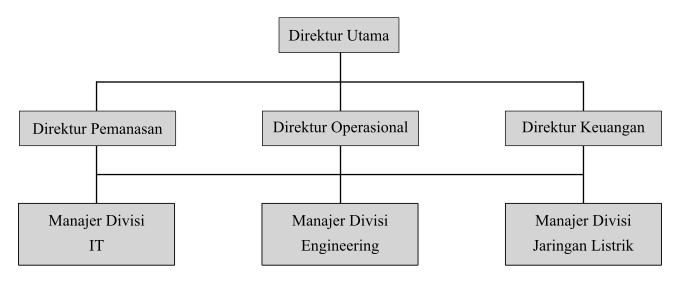
\includegraphics[width=14.5cm]{gambar/gambar_2_1.png}
    \vspace{-0.5cm}
    \captionof{figure}{\bfseries{Judul Posisi di Bawah Gambar Cetak Tebal Tanpa Titik}}
  \end{minipage}
\end{center}

% Halaman: BAB III
\chapter{METODOLOGI PELAKSANAAN KERJA PRAKTIK}

\vspace{0.5cm}

\section{Tempat dan Waktu Pelaksanaan}
Bagian ini memuat alamat tempat kerja praktik dan waktu pelaksanaan KP.

\section{Hardware dan Software}
\begin{enumerate}[label=\alph*.]
  \item Hardware\\
  Bagian ini berisi tentang hardware yang digunakan di perusahaan tempat kerja praktik.
  \item Software\\
  Bagian ini berisi tentang software yang digunakan di perusahaan tempat kerja praktik.
\end{enumerate}

\section{Metode Pengumpulan Data}
Metode deskriptif yaitu metode yang menggambarkan dan melaporkan suatu kejadian / peristiwa. Adapun teknik pengumpulan data yang digunakan :
\begin{enumerate}[label=\alph*.]
  \item Teknik Wawancara (\textit{interview})\\
    \tab[12pt] Melakukan Tanya jawab secara langsung kepada karyawan atau pegawai tempat KP.
  \item Pengamatan Langsung (\textit{observasi})\\
    \tab[12pt] Mengamati dan mempelajari secara langsung dilapangan hal- hal yang berhubungan dengan objek KP.
  \item Studi Pustaka\\
    \tab[12pt] Mencari literature yang berhubungan dengan topic laporan KP, seperti buku – buku, jurnal dan lain – lain.
\end{enumerate}

% Halaman: BAB IV
\chapter{PEMBAHASAN HASIL PELAKSANAAN KERJA PRAKTIK}

\vspace{0.5cm}

\section{Bidang Pembahasan}
Bagian ini berisi tentang bidang apa yang dianalisis / dibahas ketika melakukan kegiatan KP.

\section{Hasil Pelaksanaan / Pembahasan}
Bagian ini berisihasil pembahasan mengenai penyelesaian suatu permasalahan dibidang yang dianalisis / dibahas dari suatu perangkat / proses / metode kerja yang terdapat pada unit tempat KP.

\section{Rekomendasi (Optional)}
Bagian ini berisi tentang rekomenda siapa yang dihasil pelaksanaan KP yang dilakukan.

\noindent Contoh tabel rekomendasi :

\vspace{0.5cm}

\noindent\begin{minipage}{\textwidth}
  \label{tabel:4_1}
  \captionof{table}{\bfseries{Judul Tabel Posisi di Atas Rata Tengah Cetak Tebal Tanpa Titik}}
  \vspace{0.2cm}
  \begin{tabular}{|c|L{4cm}|L{8.5cm}|}
    \hline
    \cellcolor{Gray}\textbf{No.} & \multicolumn{1}{c|}{\cellcolor{Gray}\textbf{Hasil Analisis}} & \multicolumn{1}{c|}{\cellcolor{Gray}\textbf{Rekomendasi}}\\
    \hline
    1. & & \\
    \hline
    2. & & \\
    \hline
    3. & & \\
    \hline
    4. & & \\
    \hline
    dst. & & \\
    \hline
  \end{tabular}
\end{minipage}

% Halaman: BAB V
\chapter{PENUTUP}

\vspace{0.5cm}

\section{Kesimpulan}
Bagian ini memuat kesimpulan yang berupa rangkuman dari pelaksanaan maupun penulisan laporan dan jawaban dari rumusan masalah.

\section{Saran}
Bagian ini berisi saran – saran yang relevan berkaitan dengan hal yang sudah dituliskan dalam laporan KP, dapat juga mengenai pelaksanaan KP ataupun yang terkait dengan institusi tempat KP.

% BACK MATTER
\backmatter
\pagestyle{plain}

% Halaman: DAFTAR PUSTAKA
\chapter{DAFTAR PUSTAKA}

\vspace{0.5cm}

\begin{singlespace}
\noindent\textbf{PUSTAKA BUKU}\\

\begin{hangparas}{25pt}{1}
Nama pengarang, tahun penerbitan, judul, edisi (jika perlu), jilid (jika perlu), nama penerbit, kota penerbit.\\

Pressman, R. S., 2010, \textit{Software Engineering A Practitioner’s Approach}, Seventh Edition, McGraw Hill, New York.\\

Pressman, R. S.; Lowe,D., 2009, \textit{Web Engineering A Practitioner’s Approach}, McGraw Hill, New York.\\
\end{hangparas}

\vspace{0.5cm}

\noindent\textbf{PUSTAKA ELEKTRONIK}\\

\begin{hangparas}{25pt}{1}
Nama penulis, judul artikel, alamat URL secara lengkap, tanggal akses. Publikasi di web selain e-book, e-journal, dan e-proceeding tidak diperbolehkan untuk dijadikan rujukan.\\

Rosenberg H.,L.; Hyatt,E.,L, \textit{Software Quality Metrics for Object Oriented Environments}, Online pada \url{http://www.librarian.net/navon/ paper/SoftwareQuality_Metrics_for_Object_Oriented_Envi.pdf?paperid=1090069}, diakses tanggal 5 Januari 2015.\\
\end{hangparas}

\end{singlespace}

% Halaman: LAMPIRAN
\chapter{LAMPIRAN}

\vspace{0.5cm}

\end{document}


% BSD 2-Clause License
%
% Copyright (c) 2020, Rizqi Nur Assyaufi All rights reserved.
%
% Redistribution and use in source and binary forms, with or without
% modification, are permitted provided that the following conditions are met:
%
%   1. Redistributions of source code must retain the above copyright notice,
%      this list of conditions and the following disclaimer.
%
%   2. Redistributions in binary form must reproduce the above copyright
%      notice, this list of conditions and the following disclaimer in the
%      documentation and/or other materials provided with the distribution.
%
% THIS SOFTWARE IS PROVIDED BY THE COPYRIGHT HOLDERS AND CONTRIBUTORS "AS IS"
% AND ANY EXPRESS OR IMPLIED WARRANTIES, INCLUDING, BUT NOT LIMITED TO, THE
% IMPLIED WARRANTIES OF MERCHANTABILITY AND FITNESS FOR A PARTICULAR PURPOSE
% ARE DISCLAIMED. IN NO EVENT SHALL THE COPYRIGHT HOLDER OR CONTRIBUTORS BE
% LIABLE FOR ANY DIRECT, INDIRECT, INCIDENTAL, SPECIAL, EXEMPLARY, OR
% CONSEQUENTIAL DAMAGES (INCLUDING, BUT NOT LIMITED TO, PROCUREMENT OF
% SUBSTITUTE GOODS OR SERVICES; LOSS OF USE, DATA, OR PROFITS; OR BUSINESS
% INTERRUPTION) HOWEVER CAUSED AND ON ANY THEORY OF LIABILITY, WHETHER IN
% CONTRACT, STRICT LIABILITY, OR TORT (INCLUDING NEGLIGENCE OR OTHERWISE)
% ARISING IN ANY WAY OUT OF THE USE OF THIS SOFTWARE, EVEN IF ADVISED OF THE
% POSSIBILITY OF SUCH DAMAGE.
